\section{Versuchsaufbau}
\label{sec:versuchsaufbau}

\begin{figure}
    \centering
    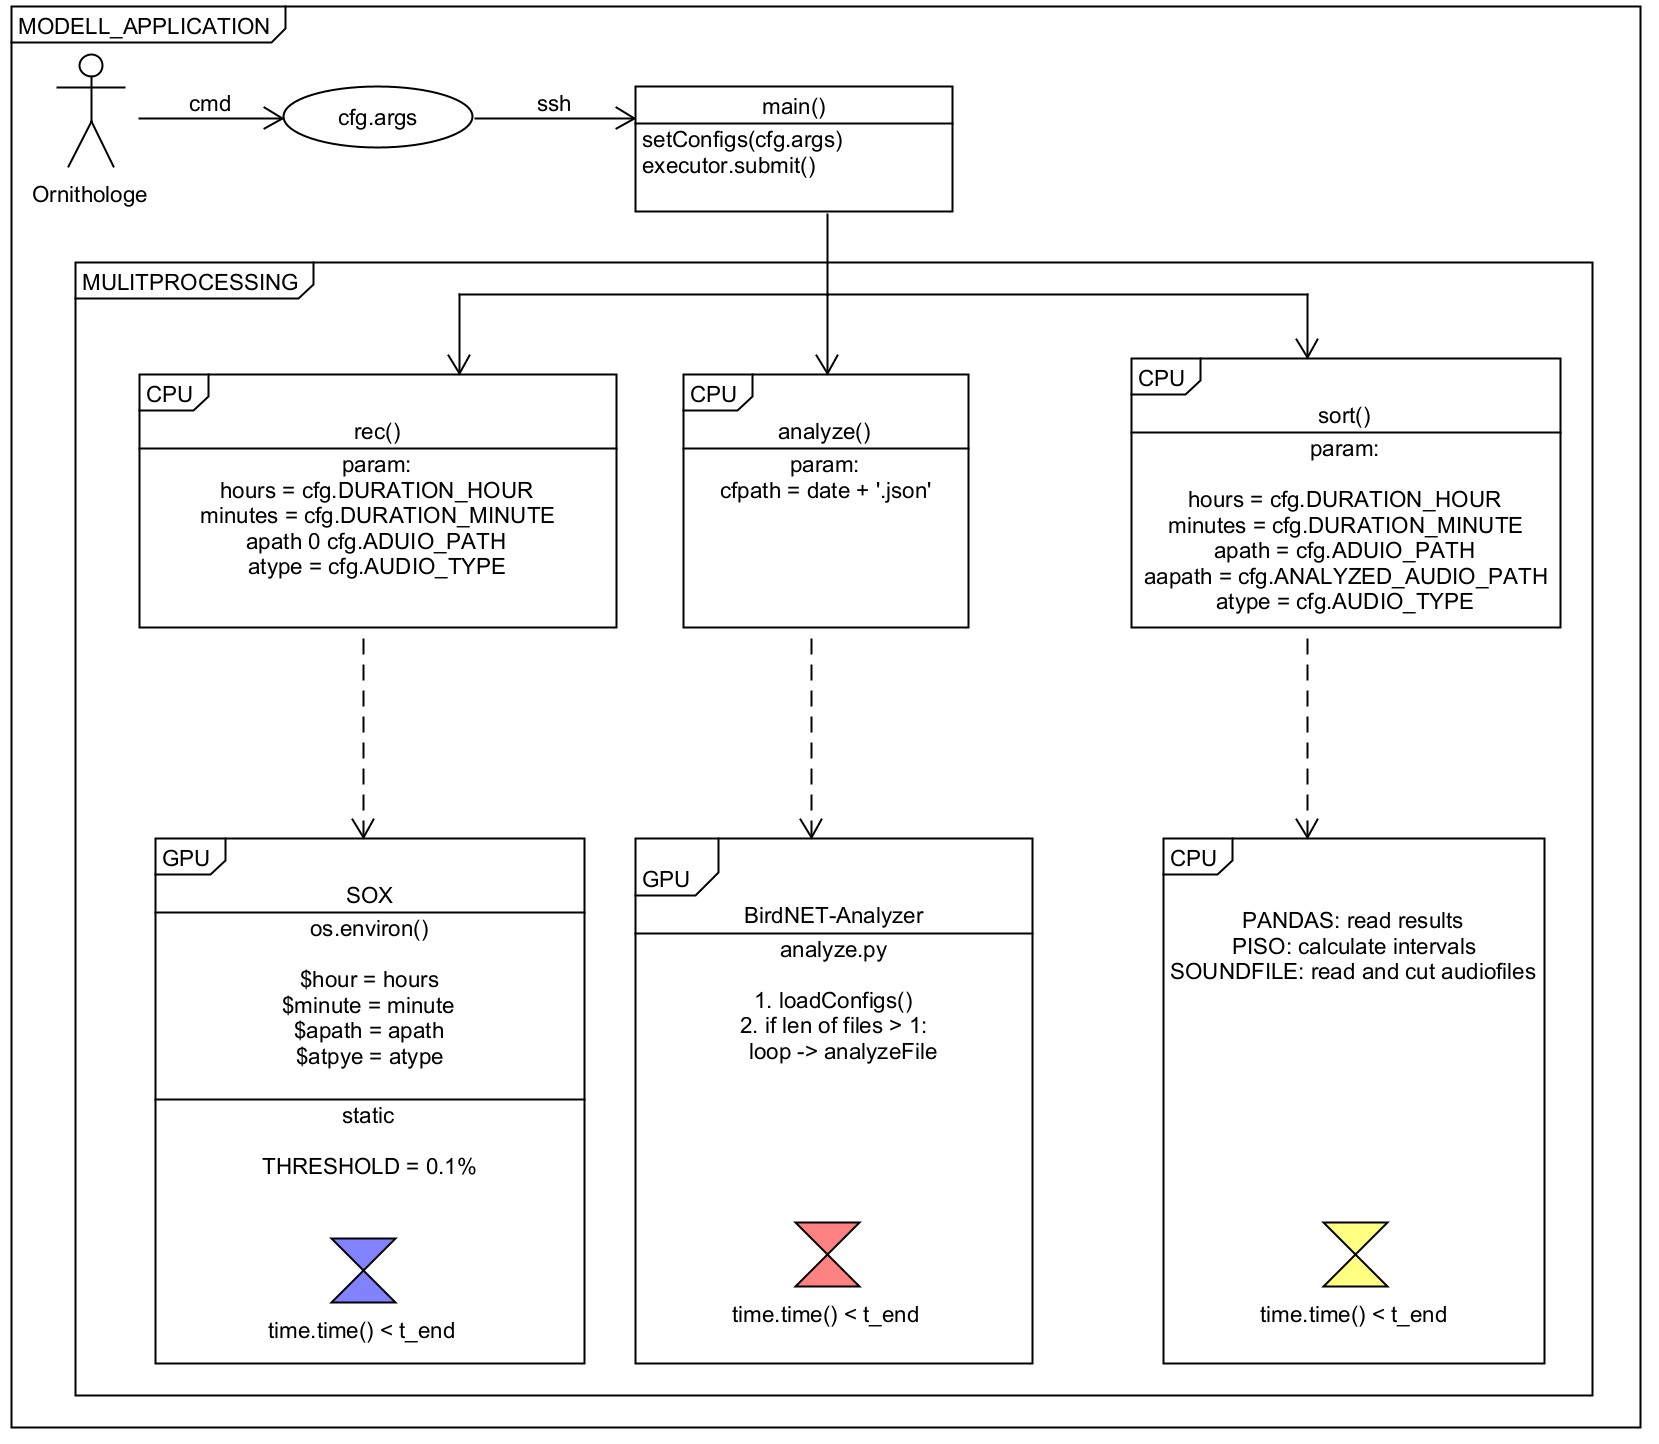
\includegraphics[width=1\linewidth]{bilder/modell_app_2.png}
 \caption{Modell der Applikation}
    \label{fig:versuchsaufbau}
\end{figure}

Das Aktivitätsdiagramm in Abbildung \ref{fig:versuchsaufbau} skizziert den Versuchsaufbau. 

Der*Die Ornithologe*in gibt manuell den Befehl auf dem lokalen Rechner ein. Der lokale Rechner ist mit dem kabellosen Netzwerk des mobilen Computers verbunden und sendet über dieses Netzwerk den Befehl an den Computer. Somit ist dieser der SSH-Server, der für die Datenannahme per SSH-Tunnel und Datenverarbeitug per Software (s. Abschnitt \ref{sec:umsetzung}) zuständig ist. Der mobile Computer ist an eine Powerstation verbunden (s. Abschnitt \ref{subsec:Stromversorgung}). Das Mikrofon ist per USB-Kabel an den Computer angeschlossen (s. Abschnitt \ref{subsec:mikrofon}).


\subsection{Computer \label{subsec:Computer}}
Als mobiler Computer kommt der Nvidia Jetson in der Version Nano J1010 zum Einsatz. 

Damit er sicher in der Box gelagert ist, sitzt er in einem Aluminiumgehäuse. Zudem ist eine Referenz-Trägerplatte von Seeed und ein passiver Aluminium-Kühlkörper eingebaut. Zur Speichererweiterung ist eine SD-Karte im Gerät hinzugefügt.

Um eine kabellose Übertragung der Daten vom Host zum Server zu ermöglichen, ist noch eine WiFi-Karte an den mobilen Computer angeschlossen (s. Abbildung \ref{fig:versuchsaufbau}).

Durch seine technischen Eigenschaften ist der Nano in seiner Performance für KI-Anwendungen geeignet. Es sei jedoch nochmal auf Abschnitt \ref{subsubsec:} hingewiesen.

Der Link zum Datenblatt befindet sich im Anhang \ref{anh:Datenblatt} \cite{jetson_datasheet}.

Alle technisch relevanten Daten sind auch auf der Seite von Nvidia gelistet \cite{jetson_web}.

Das Betriebssystem ist Linux mit Ubuntu 20.04.


\subsubsection{Nutzung eines Hardwarebeschleunigers}
\label{subsubsec:}
Ursprünglich war geplant den Nvidia Jetson Nano aufgrund seiner GPU als Hardwarebeschleuniger und der damit einhergehenden Performanceverbessung für KI-Anwen\-dung\-en zu nutzen. Jedoch hat sich im Laufe der Entwicklung dieses Projektes herausgestellt, dass Nvidia den Support, um Tensorflow %anmerkung was tensorflow ist
auf der GPU laufen zu lassen, nicht (mehr) anbietet. Auch der Umweg durch Installationsanweisungen von anderen Quellen wie von \cite{qengineering}
lohnen sich nicht, da laut diesen Quellen die GPU einen negativen Effekt auf die Rechengeschwindigkeit hat.

\subsection{Stromversorgung \label{subsec:Stromversorgung}}
Für die Stromversorgung im Freien kommt eine Powerbank zum Einsatz. Die wichtigste Anforderung an die Powerbank ist die ausreichende Stromkapazität.
Da der Jetson einen Leistungsverbrauch von 5 bis 10 Watt pro Stunde bei Auslastungen wie KI-Berechnungen oder High Perfomance Computing hat, kommt eine Powerbank mit \SI{266,4}{\watt\hour} zum Einsatz. 
%https://www.nvidia.com/de-de/autonomous-machines/embedded-systems/jetson-nano/product-development/
Durch einen praktischen Versuch ist verifiziert, dass die Stromkapazität der Powerbank ausreicht.

\subsection{Mikrofon}
\label{subsec:mikrofon}

Das Mikrofon hat die Rolle der Datenerfassung inne. Es zeichnet das umliegende Audiosignal auf und leitet es per USB-Kabel an den mobilen Computer weiter. 
Das hier gewählte Mikrofon \textsc{Clippy EM272Z1 Mono} \cite{clippy_microphone} und der dazugewählte Windschutz \cite{soundscapes_windshield} eine Empfehlung vom gekennzeichneten
Amateurfunker \cite{amateurfunker}.
Durch eigene Testversuche ist nach persönlichem Ermessen die Qualität des Mikrofons ausreichend.

%\flqq ausreichend \fqrr\ klassifiziert.


\subsubsection{GPS-Gerät}
\label{subsec:gps}
Zur Erfassung der Koordinaten ist ein GPS-Gerät angeschlossen. Diese Koordinaten verhelfen zu einer sicheren Vorhersage des Neuronalen Netzes. Zudem ermittelt es für den Computer die aktuelle Uhrzeit, da dieser %Verweis auf den Computer?
keine Echtzeit-Uhr verbaut hat. Die Nutzung der Daten vom GPS in der Software sind in Abschnitt \ref{subsec:configs} erklärt.
